%\documentclass[a4paper,superscriptaddress,11pt]{quantumarticle}
\documentclass[aps,twocolumn,longbibliography,english,superscriptaddress,prr]{revtex4-1}
%\documentclass[a4paper,superscriptaddress,11pt]{article}
\pdfoutput=1
\usepackage[colorlinks=true,urlcolor=blue,citecolor=blue,linkcolor=blue]{hyperref}
\usepackage[english]{babel}
\usepackage[utf8]{inputenc}
\usepackage[T1]{fontenc}
\usepackage{amssymb}
\usepackage{tabularx}
\usepackage{upquote}
%\usepackage{multicol}
%\usepackage{caption}
%\usepackage[plain]{algorithm}
\usepackage[ruled, vlined]{algorithm2e}
\usepackage{algpseudocode}
\usepackage{rotating}
%\usepackage{cite}
\usepackage{booktabs}
%\usepackage{unicode-math}
%\usepackage{algorithm}% http://ctan.org/pkg/algorithm
%\usepackage{algpseudocode}% http://ctan.org/pkg/algpseudocode
\usepackage{xcolor}% http://ctan.org/pkg/xcolor
\makeatletter
\newsavebox{\@brx}
\newcommand{\llangle}[1][]{\savebox{\@brx}{\(\m@th{#1\langle}\)}%
  \mathopen{\copy\@brx\kern-0.5\wd\@brx\usebox{\@brx}}}
\newcommand{\rrangle}[1][]{\savebox{\@brx}{\(\m@th{#1\rangle}\)}%
  \mathclose{\copy\@brx\kern-0.5\wd\@brx\usebox{\@brx}}}
\makeatother

\usepackage{bbm}
\usepackage{jlcode}
\usepackage{graphicx, subfigure}
\usepackage{amsmath,color,amsthm}
\usepackage{mathrsfs}
\usepackage{float}
\usepackage[normalem]{ulem}
\usepackage{indentfirst}
\usepackage{txfonts}
\usepackage[epsilon, tsrm, altpo]{backnaur}

\usepackage{listings}
\lstset{
    language=Julia,
    basicstyle=\ttfamily\footnotesize,
    numberstyle=\scriptsize,
    % numbers=left,
    backgroundcolor=\color{gray!10},
    frame=single,
    tabsize=2,
    rulecolor=\color{black!30},
    title=\lstname,
    escapeinside={\%(*}{*)},
    breaklines=true,
    breakatwhitespace=true,
    framextopmargin=2pt,
    framexbottommargin=2pt,
    extendedchars=true,
    inputencoding=utf8,
    columns=fullflexible,
}

\tolerance=1
\emergencystretch=\maxdimen
\hyphenpenalty=1000
\hbadness=1000

\makeatletter

%%%%%%%%%%%%%%%%%%%%%%%%%%%%%% User specified LaTeX commands.

%Journal reference.  Comma sets off: name, vol, page, year
\def\journal #1, #2, #3, 1#4#5#6{{\sl #1~}{\bf #2}, #3 (1#4#5#6) }
\def\pr{\journal Phys. Rev., }
\def\prb{\journal Phys. Rev. B, }
\def\prl{\journal Phys. Rev. Lett., }
\def\pl{\journal Phys. Lett., }
%\def\np{\journal Nucl. Phys., }


%%%%%%%%%%%%%%%%%%%%%%%%%%%%%%%%%%%%%%%%%%%%%%%%%%%%%%%%%%%%%%%%%%%%%%%%%%%%%%%%%%%%%%%%%%%%%%%%%%%%%%%%%%%%%%%%%%%%%%%%%%%%%%%%%%%%%%%%%%%%%%%%%%%%%%%%%%%%%%%%%%%%%%%%%%%%%%%%%%%%%%%%%%%%%%%%%%%%%%%%%%%%%%%%%%%%%%%%%%%%%%%%%%%%%%%%%%%%%%%%%%%%%%%%%%%%


%\usepackage{CJK}
%\usepackage[colorlinks, citecolor=blue]{hyperref}
\DeclareMathOperator*{\argmax}{arg\,max}

%%%%%% Shortcut related
\newcommand{\<}{\langle}
\renewcommand{\>}{\rangle}
\newcommand{\out}{{O}}
\newcommand{\inp}{{I}}
\newcommand{\pluseq}{\mathrel{+}=}
\newcommand{\minuseq}{\mathrel{-}=}
\newcommand{\vx}{{\vec x}}
\newcommand{\vg}{{\vec g}}
\newcommand{\vp}{{\vec p}}
\newcommand{\vy}{{\vec y}}
\newcommand{\vvalue}{{\texttt{value}}}
\newcommand{\grad}{{\texttt{grad}}}
\newcommand{\garbage}{{\texttt{garbage}}}
%%%%%% Convention related
\newcommand{\SWAP}{{\rm SWAP}}
\newcommand{\CNOT}{{\rm CNOT}}
\newcommand{\X}{{\rm X}}
\renewcommand{\H}{{\rm H}}
\newcommand{\Rx}{{\rm Rx}}
\renewcommand{\v}[1]{{\bf #1}}
\newcommand{\dataset}{{\mathcal{D}}}
\newcommand{\wfunc}{{\psi}}
\newcommand{\SU}{{\rm SU}}
\newcommand{\ctheta}{{\color{jlbase}{\rm \theta}}}
\newcommand{\cpi}{{\color{jlbase}{\rm \pi}}}
\newcommand{\UU}{{\rm U}}
\newcommand{\thetav}{{\boldsymbol{\theta}}}
\newcommand{\gammav}{{\boldsymbol{\gamma}}}
\newcommand{\thetai}{{\theta^\alpha_l}}
\newcommand{\Expect}{{\mathbb{E}}}
\newcommand{\Tr}{{\rm Tr}}
\newcommand{\etc}{{\it etc~}}
\newcommand{\etal}{{\it etal~}}
\newcommand{\xset}{\mathbf{X}}
\newcommand{\fl}{\texttt{fl}}
\newcommand{\pdata}{\mathbf{\pi}}
\newcommand{\q}{\mathbf{q}}
\newcommand{\epdata}{\mathbf{\hat{\pi}}}
\newcommand{\gammaset}{\boldsymbol{\Gamma}}
\newcommand{\ei}{{\mathbf{e}_l^\alpha}}
\newcommand{\vtheta}{{\boldsymbol{\theta}}}
\newcommand{\sigmag}{{\nu}}
\newcommand{\sigmai}[2]{{\sigma^{#2}_{#1}}}
\newcommand{\qi}[1]{{q^{\alpha_{#1}}_{#1}}}
\newcommand{\BAS}{Bars-and-Stripes}
\newcommand{\circled}[1]{\raisebox{.5pt}{\textcircled{\raisebox{-.9pt} {#1}}}}

\newcommand{\qexpect}[1]{{\left\langle #1\right\rangle}}
\newcommand{\expect}[2]{{\mathop{\mathbb{E}}\limits_{\substack{#2}}\left[#1\right]}}
\newcommand{\var}[2]{{\mathop{\mathrm{Var}}\limits_{\substack{#2}}\left(#1\right)}}
\newcommand{\pshift}[1]{{p_{\thetav+#1}}}
\newcommand{\upcite}[1]{\textsuperscript{\cite{#1}}}
\newcommand{\Eq}[1]{Eq.~(\ref{#1})}
\newcommand{\Fig}[1]{Fig.~\ref{#1}}
\newcommand{\Tbl}[1]{Table~\ref{#1}}
\newcommand{\Sec}[1]{Sec.~\ref{#1}}
\newcommand{\App}[1]{Appendix \ref{#1}}
\newcommand{\bra}[1]{\mbox{$\left\langle #1 \right|$}}
\newcommand{\ket}[1]{\mbox{$\left| #1 \right\rangle$}}
\newcommand{\braket}[2]{\mbox{$\left\langle #1 | #2 \right\rangle$}}
\newcommand{\tr}[1]{\mathrm{tr}\mbox{$\left[ #1\right]$}}

\newcommand{\ra}[1]{\renewcommand{\arraystretch}{#1}}

%%%%%% Comment related
\newcommand{\red}[1]{[{\bf  \color{red}{LW: #1}}]}
\newcommand{\xred}[1]{[{\bf  \color{red}{\sout{LW: #1}}}]}
\newcommand{\blue}[1]{[{\bf  \color{blue}{JG: #1}}]}
\newcommand{\green}[1]{[{\bf  \color{green}{TZ: #1}}]}
\newcommand{\xgreen}[1]{[{\bf  \color{green}{\sout{TZ: #1}}}]}
\newcommand{\xblue}[1]{[{\bf  \color{blue}{\sout{JG: #1}}}]}
\newcommand{\material}[1]{\iffalse[{\bf  \color{cyan}{Material: #1}}]\fi}

\newtheorem{theorem}{\textit{Theorem}}
\theoremstyle{definition}\newtheorem{definition}{\textit{Definition}}

\makeatother

\begin{document}
\title{Instruction level automatic differentiation on a reversible Turing machine}

%\author{Jin-Guo Liu\thanks{cacate0129@iphy.ac.cn}\\
%Institute of Physics, Chinese Academy of Sciences,\\Beijing 100190, China\\
%\And
%Hong-Xuan Zhao-Wang\\
%Department of Computer Science, University of Tsukuba
%}
%\author{Lei Wang}
%\email{wanglei@iphy.ac.cn}
%\affiliation{Institute of Physics, Chinese Academy of Sciences, Beijing 100190, China}
%\affiliation{CAS Center for Excellence in Topological Quantum Computation, University of Chinese Academy of Sciences, Beijing 100190, China}
%\affiliation{Songshan Lake Materials Laboratory, Dongguan, Guangdong 523808, China}

\author{Jin-Guo Liu}
\email{cacate0129@iphy.ac.cn}
\affiliation{Institute of Physics, Chinese Academy of Sciences, Beijing 100190, China}

\author{Taine Zhao}
\affiliation{Department of Computer Science, University of Tsukuba}

\begin{abstract}
    This paper considers the instruction level adjoint mode automatic differentiation. Here, instruction level means, given the backward rules of basic instructions like +, -, * and /, one can differentiate an arbituary program efficiently. In this paper, we review briefly why instruction level automatic differentiation is hard for traditional machine learning frameworks and propose a solution to these problems by back propagating a reversible Turing machine. This implementation can be used to generate the backward rules for functions from exp to unitary matrix multiplication and QR decomposition. Also we discuss the challenges that we face towards a rigorious reversible programing from the instruction and hardware perspective.
\end{abstract}


\maketitle

%\begin{multicols}{2}
\section{Introduction}\label{sec:intro}
    There are two modes of automatic differentiation (AD)~\cite{Hascoet2013}, the tangent mode and the adjoint mode.
    Consider a multi-in multi-out function $\vy = f(\vx)$, the tangent mode computes one column of its Jacobian $\frac{\partial \vy}{\partial x_i}$ efficiently, where $x_i$ is one of the input variables.
Whereas the adjoint mode computes one row of Jacobian $\frac{\partial y_i}{\partial \vec{x}}$ efficiently.
Most popular automatic differentiation packages implement the adjoint mode AD. Because the adjoint mode is computational more efficient in variational applications, where the loss as output is always a scalar.
However, implementing adjoint mode AD is harder than implementing its tangent mode counterpart. It requires a program's intermediate state for back propagation, which includes
\begin{enumerate}
    \item the computational graph,
    \item and input variables of nodes in computational graph.
\end{enumerate}
    A computational graph is a directed acyclic graph (DAG) that records the relation between data (edges) and functions (nodes).
In Pytorch~\cite{Paszke2017} and Flux~\cite{Innes2018}, every variable has a tracker field that stores its parent information, i.e. the input data and function that generate this variable. TensorFlow~\cite{Tensorflow2015} implements a static computational graph as a description of the program before actual computation happens.
    Source to source automatic differentiation package Zygote~\cite{Innes2018, Innes2019} use a intermediate representation (IR) of a program, the static single assignment (SSA) form, as the computational graph in order to back propagate a native julia code. To cache intermediate states, it has to accesss a global storage.

    Several limitations are observed in these AD implementions due to the recording and caching. First of all, these package requires a lot primitive functions with programmer defined backward rules. This is not nessesary given the fact that, at the lowest level, these primitive functions are compiled to a finite set of instructions including `+', `-', `*', `/' and conditional jump. By defining backward rules for these basic instructions, AD should just works. These machine learning packages can not use instructions as the computational graph for practical reasons. The cost of memorizing the computational graph and caching intermediate states is huge. It can decrease the performance for more than two orders when a program contains loops (as we will show latter).
    Even more, the memory consumption for caching intermediate results increases linearly as time. In many deep learning models like recurrent neural network~\cite{Lipton2015} and residual neural networks~\cite{He2016}, the depth can reach several thousand. The memory is often the bottleneck of these programs, which is known as the memory wall problem.~\cite{memorywall}
    Secondly, inplace functions are not handled properly in the diagram of computational graph, because the notation of parent and child are not compatible with inplace operations.
 Even in Zygote that uses SSA as the computational graph, it is not trivil to handle inplace functions.
    On the other side, most functions in BLAS and LAPACK are implemented as inplace functions. All AD packages that use BLAS and LAPACK functions have to define their own backward rules for their non-inplace wrappers due to the lack of AD support to inplace functions.
    Thridly, obtaining higher order gradients are not efficient in these packages. For example, in most machine learning packages, people back propagate the whole program of obtaining first order gradients to obtain second order gradients. The repeated use of back propagation cause an exponential overhead with respect to the order of gradients. A better approach is using Taylor propagation like in JAX~\cite{Bettencourt2019}. However Taylor propagation requires writing backward rules for all primitives\blue{true?}. %Besides the exponential overhead, the sorce to source AD engine Zygote suffers from the significant overhead of just in time compiling in Julia language~\cite{Bezanson2017}.

% where the manually derived backwards rule still faces the degenerate spectrum problem (gradients explodes), instruction level AD will return reasonable gradients. With instruction level AD, people don't worry about inplace functions, which may be a huge problem in traditional approaches. We can back propagate over a quantum simulator, where all instructions are reversible two level unitaries (i.e. Jacobian rotation).

%We don't need extra effort to learn meta parameters.~\cite{} Neural ODE is much easier to design~\cite{Chen2018}.

Our solution to these issues is making a program time reversible. It is not same as the work arounds in the machine learning field that use information buffer~\cite{Maclaurin2015} and reversible activation functions to reduce the memory allocations in recurrent neural network~\cite{MacKay2018} and residual neural networks~\cite{Behrmann2018}. Our approach is more general, we develop a embeded domain specific language (eDSL) in Julia language that implements reversible Turing machine (RTM).~\cite{Perumalla2013,Frank2017}.
The gradient of any program written in this eDSL can be obtained in comparable time with the forward computation. The AD implementation is similar to \texttt{ForwardDiff}~\cite{Revels2016} but runs backward.
    In history, there has been some prototypes of reversible languages like Janus~\cite{Lutz1986}, R (not the popular one)~\cite{Frank1997}, Erlang~\cite{Lanese2018} and object oriented ROOPL~\cite{Haulund2017}. These languages have reversible control flow that allows user to input an additional postcondition in control flows to help programs run backward.
    In the past, the main motivation of making a program time reversible is to support reversible devices. Reversible devices do not have a lower bound of energy consumption by Landauer principle~\cite{Landauer1961}. However, people show less and less interest to reversible programming since 15 years ago since the energy efficiency of CMOS devices are still two orders~\cite{Frank2017} above this lower bound, this lower bound is not an urgent problem yet.
    The main contribtion of our work is breaking the information barrier between machine learning community and reversible programming community, providing yet another strong motivation to develop reversible programming.
    Our eDSL borrows the design of reversible control flow in the Janus, meanwhile provides multiple dispatch based abstraction. With these features, the AD engine could be implemented in less than 100 lines. It generates native julia code, and is completely compatible with Julia language.
Potensial applications includes
\begin{enumerate}
    \item generate AD rules for primitive functions like \texttt{exp},
    \item control problem in robotics~\cite{Giftthaler2017} where tensor is not the dominating data type,
    \item differentiating over reversible integrators~\cite{Laikov2018} without intermediate state caching,
    \item Stablize the backward rules for linear algebra functions. Current backward rules for singular value decomposition (SVD) and eigenvalue decomposition (ED)~\cite{Seeger2017,Wan2019,Hubig2019} are vulnarable to spectrum degeneracy. The development of backward rules for these linear algebra functions can greatly change researches in physics~\cite{Xie2020,Liao2019}.

\end{enumerate}

    In this paper, we first introduce the design of our eDSL in \Sec{sec:lang}.
    In \Sec{sec:bp}, we show how to back propagation Jacobians and Hessians in a reversible programming language.
    We propose a self consistent training strategy in \Sec{sec:train} that utilizes reversibility directly, which does require gradients.
    In \Sec{sec:example}, we show several examples.
    In \Sec{sec:discussion}, we discuss on several important issues, how time space tradeoff works, reversible instructions and hardwares and finally an outlook to some open problems to be solved.

\section{Language design}\label{sec:lang}
    \green{This is an example of comment!}
We instroduce NiLang, a eDSL in Julia that simulates RTM. Its grammar is shown in \App{app:grammar}.
Its main feature is contained in a single macro \texttt{@i}. It interprets a NiLang function to a native Julia function.
At the same time, it generates the inverse of this function. The target instructions are closed under the inverse operation ``$\sim$'', hence all functions defined in NiLang are also closed under ``$\sim$'' operations.

    In a mordern programming language, functions are pushed to a global stack for scheduling. The memory layout of a function is consisted of input arguments, a function frame with informations like return address and saved memory segments, local variables and working stack. After each call, the function clears the input arguments, function frame, local variables and working stack, only stores the return value.
    In the reversible programming style, this kind of design pattern is nolonger the best practise, input variables can not be easily discarded after a function call, since discarding information may ruin reversibility. Hence, a function or a instruction changes inputs "inplace" in NiLang.
To design such a eDSL, we first introduce a reversible IR that plays a central role in NiLang.

\subsection{Reversible IR}

\begin{figure}
    \centerline{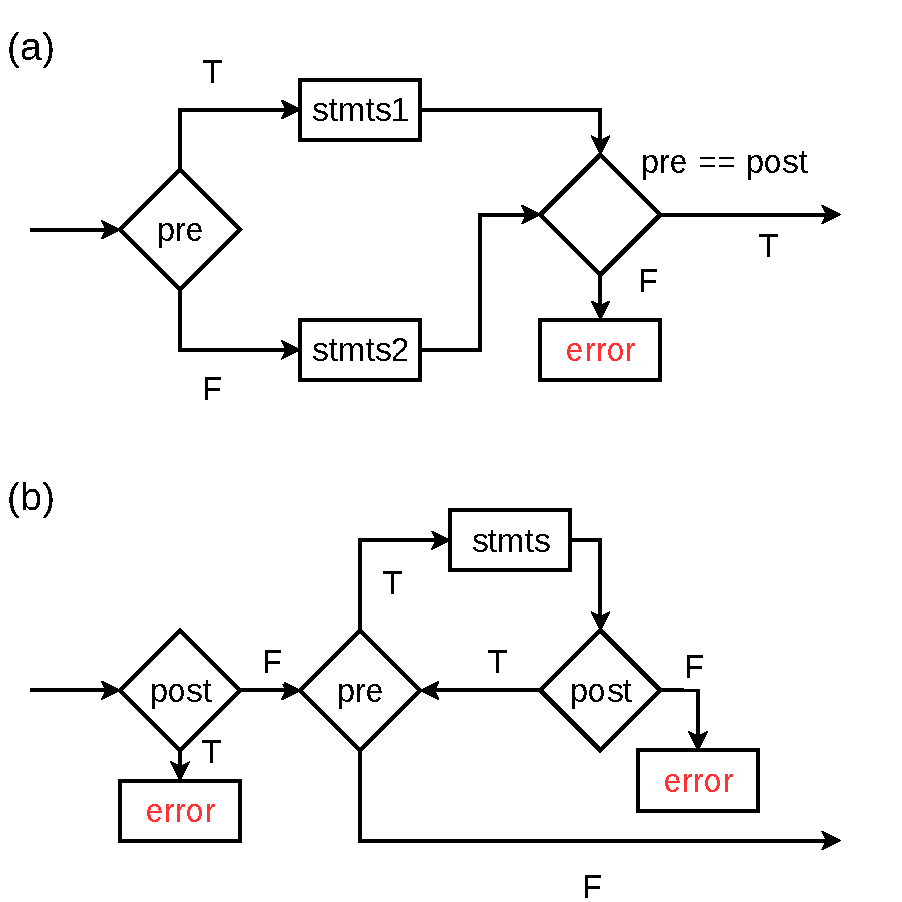
\includegraphics[width=0.8\columnwidth,trim={0 0cm 0 0cm},clip]{images/controlflow.pdf}}
    \caption{Flow chart for reversible (a) \texttt{if} statement and (b) \texttt{while} statement. ``stmts'', ``stmts1'' and ``stmts2'' are statements, statements in true branch and statements in false branch respectively. ``pre'' and ``post'' are precondition and postconditions respectively. ``error'' refers to \texttt{InvertibilityError}.}\label{fig:controlflow}
\end{figure}

\begin{table}[h!]\centering
\begin{minipage}{\columnwidth}
\ra{1.3}
    \scalebox{1.0}{
        \begin{tabularx}{\textwidth}{X X}\toprule
            \textbf{statement} & \textbf{inverse}\\
            \hline
            \texttt{<f>(<args>...)} & \texttt{($\sim$<f>)(<args>...)}\\
            \hline
            \texttt{<y!> += <f>(<args>...)} & \texttt{<y!> -= <f>(<args>...)}\\
            \hline
            \texttt{<y!> .+= <f>.(<args>...)} & \texttt{<y!> .-= <f>.(<args>...)}\\
            \hline
            \texttt{<y!> $\veebar$= <f>(<args>...)} & \texttt{<y!> $\veebar$= <f>(<args>...)}\\
            \hline
            \texttt{<y!> .$\veebar$= <f>(<args>...)} & \texttt{<y!> .$\veebar$= <f>(<args>...)}\\
            \hline
            \texttt{@anc <a> = <expr>} & \texttt{@deanc <a> = <expr>}\\
            \hline
            \texttt{begin\newline $_\quad$<stmts>\newline end} & \texttt{begin\newline $_\quad$ $\sim$(<stmts>)\newline end}\\
            \hline
            \texttt{if (<pre>, <post>)\linebreak $_\quad$<stmts1>\newline else\newline $_\quad$<stmts2>\newline end} & \texttt{if (<post>, <pre>)\newline $_\quad$$\sim$(<stmts>)\newline else\newline $_\quad$ $\sim$(<stmts>)\newline end}\\
            \hline
            \texttt{while (<pre>, <post>)\newline $_\quad$<stmts> \newline end} & \texttt{while (<post>, <pre>)\newline $_\quad$ $\sim$(<stmts>)\newline end}\\
            \hline
            \texttt{for <i>=<m>:<s>:<n>\newline $_\quad$<stmts>\newline end} & \texttt{for <i>=<m>:-<s>:<n>\newline $_\quad$ $\sim$(<stmts>)\newline end}\\
            \hline
            \texttt{@safe <expr>} & \texttt{@safe <expr>}\\
            \bottomrule
        \end{tabularx}
    }
    \caption{A collection of reversible statements.}\label{tbl:revstatements}
\end{minipage}
\end{table}

In NiLang's IR, a statement can be an instruction, a function call, a controlflow, a macrocall or the inverse statement $\sim$.
With the reversible IR, the inverse of a statement can be defined easily as shown in  in \Tbl{tbl:revstatements}.
%For example, an instruction \texttt{y! $\mathrel{+}=$ f(args...)} is interpreted as a julia function call \texttt{PlusEq(f)(y!, args...)} or \texttt{$\oplus$(f)(y!, args...)} as a shorthand.
%Here, the ``!'' after a variable is used as a convension to indicate that a variable is changed after the call of an instruction or function.
%The detailed specification of instructions is listed in \App{app:instr}. The function call is same as the host language, except every function \texttt{f} has a \texttt{$\sim$f} that binded to an object of type \texttt{Inv\{typeof(f)\}}. \texttt{$\sim$f} invokes the compiled inverse functions of \texttt{f}.

The reversible control flow is different from the irreversible one that a condition expression in a \texttt{if} or a \texttt{while} statements is a two-element tuple that consist of a precondition and a postcondition. This design allows user putting additional postcondition in control flows to help reverse the program.
%A postcondition is a boolean expression that being evaluated after the body expressions being executed.
For the \texttt{if} statement as shown in \Fig{fig:controlflow} (a), the program enters the branch specified by precondition. After executing this branch, the program checks the consistency of precondition and postcondition to make sure they are same. In the reverse pass, the program enters the branch specified by the postcondition.
For the \texttt{while} statement as shown in \Fig{fig:controlflow} (b), before entering, the program check the postcondition to make sure it is false.
After each iteration, the program asserts the postcondition to be true. The inverse function exchanges the precondition and postcondition.
The definition of reversible \texttt{for} statement is similar to irreversible ones except it is more restrictive.
The program first stores the loop informations, start, step and stop. After the executing the loop, the program checks the values of these variables to make sure they are not changed. The reverse program exchanges start and stop and inverse the sign of step.

    There is no assign statements in a reversible language, a reversible replacement is the macro \texttt{@anc}. \texttt{@anc a = <expr>} binds variable \texttt{a} to an initial value specified by \texttt{<expr>}. Its inverse \texttt{@deanc a = <expr>} deallocates the variable \texttt{a}. Before deallocating the variable, the program checks that the value of variable is same as the value of \texttt{<expr>}, otherwise throws an \texttt{InvertibilityError}. \texttt{@anc} and \texttt{@deanc} must appear in pairs inside a function call, a while statement or a for statement.
    \texttt{@deanc} will be added automatically. Similar designs in Janus and R are \texttt{local/delocal} statement and \texttt{let} statement.
    The additional check underlines the difference between the irreversible assign statement and reversible ancilla statement.
The \texttt{@safe} macro can be followed by an arbituary statement, it allows user to use external statements that does not break reversibility.
For example, one can use \texttt{@safe @show var} for debugging.

\subsection{Compiling}
The interprecation of a reversible function consists three stages.
The first stage preprocess human inputs to a reversible IR, 
The second stage generates the reversed IR according to table \Tbl{tbl:revstatements}.
The third stage is translating this reversible IR to native Julia code.
The following example shows how to compile an \texttt{if} statement

\begin{minipage}{.44\textwidth}
\begin{lstlisting}
julia> using NiLangCore, MacroTools

julia> ex0 = :(if (x > 3, ~)
            -arr[3].value += x * y
        end);
        
julia> ex0 |> prettify
:(if (x > 3, ~)
      -(arr[3]).value += x * y
  end)

julia> ex1 = NiLangCore.precom_ex(ex0,
        NiLangCore.PreInfo());
        
julia> ex1 |> prettify  # after stage 1
:(if (x > 3, x > 3)
      -(arr[3]).value += x * y
  else
  end)

julia> ex2 = NiLangCore.dual_ex(ex1);

julia> ex2 |> prettify  # after stage 2
:(if (x > 3, x > 3)
      -(arr[3]).value -= x * y
  else
  end)

julia> ex3 = NiLangCore.interpret_ex(ex2);

julia> ex3 |> prettify  # after stage 3
quote
    wren = x > 3
    if wren
        @instr -(arr[3]).value -= x * y
    else
    end
    @invcheck x > 3 wren
end
\end{lstlisting}
\end{minipage}

In the first stage, the preprocessor expands the symbol \texttt{$\sim$} in postcondition field of \texttt{if} statement to the precondition as shown above. Besides, it adds missing \texttt{@deanc} to ensure \texttt{@anc} and \texttt{@deanc} statements appear in pairs and  expands \texttt{@routine} macro.
\texttt{@routine r <stmt>} records a statement to symbol \texttt{r}. When \texttt{$\sim$@routine r} is called, the inverse statement is inserted to that position for uncomputing. We will use macro extensively in the example in \Sec{sec:example}.
In the last stage, the compiler adds \texttt{@instr} before each instruction and function call statement.
The macro \texttt{@instr} assign the output of a function to the argument list of a function. We will explain this macro in detail in next subsection.
It also adds statements to check the consistency between preconditions and postconditions to ensure reversibility.
In the above example, \texttt{@invcheck x > 3 wren} will throw an error if the variable \texttt{wren} and \texttt{x > 3} are not equivalent.
Finally, at the end of a function body, it attaches a return statement that uses input variables as the output.
Now the function is ready to execute on the host language.

\subsection{Types and Dataviews}
So far, the language design is not too different from a tranditional reversible language.
Next, we introduce type and dataviews that are important to the implementation of adjoint mode AD.

The constructor of a type is a reversible function.
Its inverse function is a ``destructor'', which does not deallocate memory directly but unpacks data.
One can use \texttt{@iconstruct} to define a reversible constructor.
For example, we can define a type that copies the input data to a new field.

\begin{minipage}{.44\textwidth}
\begin{lstlisting}
using NiLangCore, Test

struct DVar{T}
    x::T
    g::T
end

@iconstruct function DVar(xx, gg=zero(xx))
    gg += identity(xx)
end

@test (~DVar)(DVar(0.5)) == 0.5
\end{lstlisting}
\end{minipage}

Here, the \texttt{@iconstruct} generates a reversible constructor with single parameters \texttt{xx} as input. The statement \texttt{gg = zero(xx)} initializes a new memory to be used. The body of function is a reversible program that modifies \texttt{xx} and \texttt{gg} reversiblely. Finally it calls the default constructor \texttt{DVar(xx, gg)}. It is easy to define the inverse procedure that transform a \texttt{DVar\{T\}} instance to a \texttt{T} instance by reversing the statements. With the flexibility to use types, it is not nessesary to use global stacks in our eDSL.

Before introducing dataviews, let's first consider the following line that appear in the last subsection

\begin{minipage}{.44\textwidth}
\begin{lstlisting}
-arr[3].value += x * y
\end{lstlisting}
\end{minipage}

In Julia, this statement will raise a syntax error, since a function call \texttt{(-)} can not be assigned.
Meanwhile \texttt{arr[3]} might be a immutable type.
In our eDSL, we wish it works because every memory cell should be modifiable ``inplace''.
As we have mensioned, \texttt{-arr[3].value += x * y} is translated to \texttt{@instr -arr[3].value += x * y} at the thrid stage.
\texttt{@instr} translate the statement to

\begin{minipage}{.44\textwidth}
    \begin{lstlisting}[numberstyle=\scriptsize\color{codegray},numbers=left,numbersep=8pt]
res = PlusEq(*)(-arr[3].value, x, y)
arr[3] = chfield(arr[1], Val(:value), 
    chfield(arr[3].value, -, res[1]))
x = res[2]
y = res[3]
\end{lstlisting}
\end{minipage}

\texttt{PlusEq(*)(-arr[3].value, x, y)} computes the output, which is a tuple of length $3$.
The assignments in line 4 and 5 can be handled directly while the assignment in line 2-3 are not so, where \texttt{chfield} is used to modify a dataview.
A dataview of a data can be data itself, a field of its view, an array element of its view, or a bijective mapping of its view.
\texttt{chfield(x, Val\{:value\}, val)} can modify the \texttt{value} field of an instance given the default constructor of a type is not overwritten.
A bijective mapping of a field can also be modified. To change \texttt{-x}, one simply overwrite the \texttt{chfield(x, -, res[1])} function.

\section{Automatic differentiation}\label{sec:bp}

\subsection{First order gradient}\label{sec:jacobian}
Given a node $\vec y = f(\vec x)$ in a computational graph,
%the tangent mode AD propagates the Jacobians like
%\begin{align}
%    J^{\vy}_{\inp_j} = J^{\vy}_{\vx} J_{\inp_j}^{\vx}.
%\end{align}
%$\inp$ is the inputs and 
%whereas the 
the adjoint mode AD propagates the Jacobians in the reversed direction like
\begin{align}
    \begin{split}
        J^{\out}_{\out'} &= \delta_{\out,\out'}\\
        J^{\out}_{x} &= J^{\out}_{y} J^{y}_{x},
    \end{split}
\end{align}
where $\out$ represents the outputs of the program, $J^{\out}_{x/y}$ is the adjoint to be propagated, and $J^{y}_x$ is the local Jacobian matrix. Einstein's notation is used so that duplicated indices are summed over.
%Tagent mode instruction level automatic differentiation can be implemented easily in a irreversible language with dual numbers~\cite{Revels2016}.
%Here we focus on the adjoint mode.
This back propagation rule can be rewritten in the language of tensor networks~\cite{Orus2014} as shown in \Fig{fig:ad}.
\begin{figure}
    \centerline{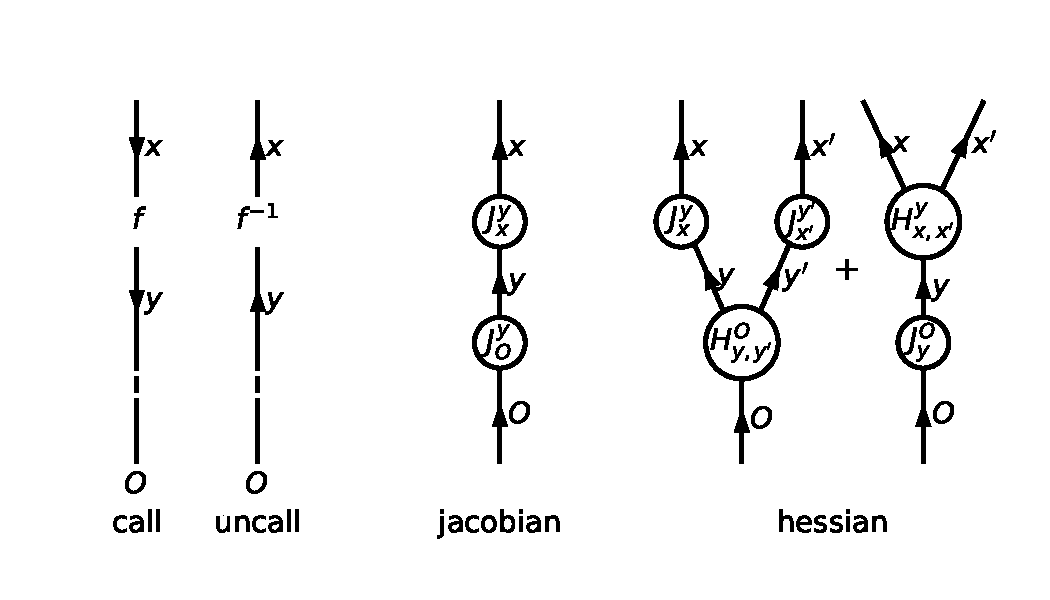
\includegraphics[width=0.9\columnwidth,trim={0.5cm 1cm 0 1cm},clip]{images/ad.pdf}}
    \caption{Adjoint rules for Jacobians and Hessians in tensor network language.}\label{fig:ad}
\end{figure}

In reversible programming with multiple dispatch, the adjoint mode AD algorithms can be implemented as

\begin{algorithm}[H]
    \KwResult{\grad.($\vx_g$)}
    let \texttt{iloss} be the index of loss variable in $\vx$\\
    $\vy = f(\vx)$\\
    $\vy_g$ = \texttt{GVar}.($\vy$)\\
    \grad($\vy_g$[\texttt{iloss}]) += 1.0\\
    $\vx_g= f^{-1}(\vy_g)$
    \caption{Reversible programming AD}\label{alg:ad}
\end{algorithm}

Here, \texttt{GVar} is a reversible type. The constructor attaches a zero gradient field to a variable, which is similar to the dual number in tangent mode automatic differentiation~\cite{Revels2016}. If the input is an array, \texttt{GVar} will be broadcasted to each array element. The gradient field of a \texttt{GVar} instance can be accessed by the \texttt{grad} dataview. Its inverse \texttt{$\sim$GVar} deallocates the gradient field safely and returns its value field. Here, "safely" means before deallocation, the program will check the gradient field to make sure its value is restored to $0$.
When an instruction \texttt{instruct} meets a \texttt{GVar}, besides computing its value field $\vvalue(\vy) = \texttt{instruct}(\vvalue(\vx))$, it also updates the gradient field $\grad(\vy) = \left[J^{\vy}_{\vx}\right]^{-1} \grad(\vx)$, where $\left[J^{\vy}_{\vx}\right]^{-1}$ is the Jacobian of $\texttt{instruct}^{-1}$. One can define this gradient function on either \texttt{instruct} or \texttt{instruct${}^{-1}$}, NiLang will generate the backward rule for the inverse function automatically. As an example, We bind the adjoint function of \texttt{ROT} to its reverse \texttt{IROT} by defining a new function that dispatch to \texttt{GVar}

\begin{minipage}{.44\textwidth}
    \begin{lstlisting}[mathescape=true]
@i function IROT(a!::GVar, b!::GVar, $\ctheta$::GVar)
    IROT(value(a!), value(b!), value($\ctheta$))
    NEG(value($\ctheta$))
    value($\ctheta$) -= identity($\cpi$/2)
    ROT(grad(a!), grad(b!), value($\ctheta$))
    grad($\ctheta$) += value(a!) * grad(a!)
    grad($\ctheta$) += value(b!) * grad(b!)
    value($\ctheta$) += identity($\cpi$/2)
    NEG(value($\ctheta$))
    ROT(grad(a!), grad(b!), $\cpi$/2)
end
\end{lstlisting}
\end{minipage}

The definition of \texttt{ROT} instruction could be found in \Sec{app:instr}. This backward rule has been included in NiLang, one can check the gradients by typing in a Julia REPL
%When gradients are not used anymore, the reversible way to deallocate gradients is uncomputing the whole process of obtaining them.
%, which increases the hyrachy by 1. Whenever the hyrachy increase by 1, the computational overhead doubles comparing with its irreversible counter part.

\begin{minipage}{.44\textwidth}
    \begin{lstlisting}[mathescape=true]
julia> using NiLang, NiLang.AD

julia> x, y, $\ctheta$ = GVar(0.5), GVar(0.6), GVar(0.9)
(GVar(0.5, 0.0), GVar(0.6, 0.0)), GVar(0.9, 0.0)

julia> @instr grad(x) += identity(1.0)

julia> @instr ROT(x, y, $\ctheta$)

julia> x, y, $\ctheta$
(GVar(-0.1591911616411577, 0.6216099682706646),
 GVar(0.7646294357761403, 0.7833269096274833),
 GVar(0.8999999999999999, 0.6))
\end{lstlisting}
\end{minipage}


The implementation of Algorithm \ref{alg:ad} is so short that we present the function defintion as follows

\begin{minipage}{.44\textwidth}
\begin{lstlisting}
@i function (g::Grad)(args...; kwargs...)
    @safe @assert count(x -> x isa Loss, args) == 1
    @anc iloss = 0
    @routine getiloss begin
        for i=1:length(args)
            if (tget(args,i) isa Loss, iloss==i)
                iloss += identity(i)
                (~Loss)(tget(args,i))
            end
        end
    end

    g.f(args...; kwargs...)
    GVar.(args)
    grad(tget(args,iloss)) += identity(1.0)
    (~g.f)(args...; kwargs...)

    ~@routine getiloss
end
\end{lstlisting}
\end{minipage}

Input variables must contain exactly one \texttt{Loss} instance.
This program first checks the input parameters and locate the loss variable as \texttt{iloss}. Then \texttt{~Loss} unwraps the loss variable.
After computing the forward pass and backward pass, \texttt{~@routine getiloss} uncomputes the ancilla \texttt{iloss} and returns the location information to the target variable.
\texttt{tget(args, i)} is used to get the $i$-th element of a tuple.
In NiLang, array indexing are supported. To avoid confusion, tuple indexing is forbidden delebrately.

The overhead of using \texttt{GVar} type can be removed thanks to Julia's multiple dispatch and type inference. Let's consider a simple example that acccumulate $1.0$ to a target variable $x$ for $n$ times

\begin{minipage}{.44\textwidth}
\begin{lstlisting}
julia> using NiLang, NiLang.AD, BenchmarkTools

julia> @i function prog(x, one, n::Int)
           for i=1:n
               x += identity(one)
           end
       end

julia> @benchmark prog'(Loss(0.0), 1.0, 10000)
BenchmarkTools.Trial: 
  memory estimate:  1.05 KiB
  allocs estimate:  39
  --------------
  minimum time:     35.838 μs (0.00% GC)
  median time:      36.055 μs (0.00% GC)
  mean time:        36.483 μs (0.00% GC)
  maximum time:     185.973 μs (0.00% GC)
  --------------
  samples:          10000
  evals/sample:     1
\end{lstlisting}
\end{minipage}

\begin{figure}
    \centerline{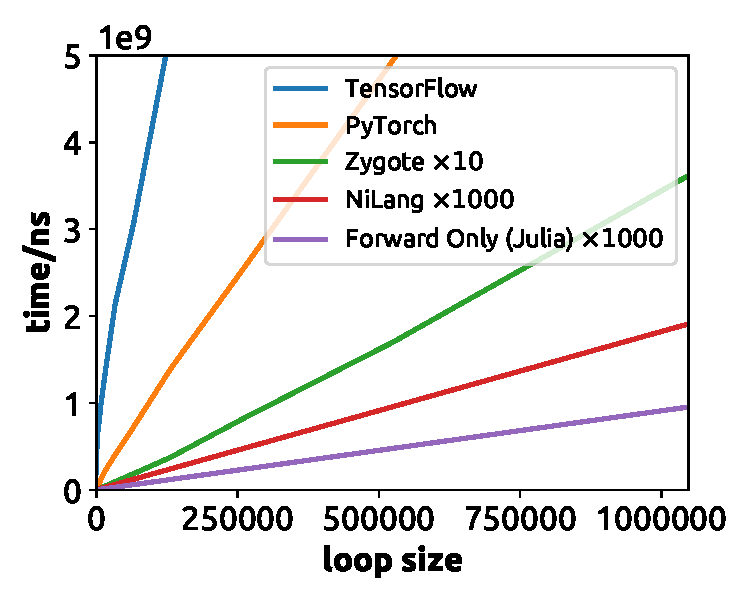
\includegraphics[width=0.9\columnwidth,trim={0 0cm 0 0},clip]{images/fig3.pdf}}
    \caption{The time for obtaining gradient as function of loop size. $\times n$ in lengend represents a rescaling of time.}\label{fig:benchmark}
\end{figure}
We implement the same function with TensorFlow, PyTorch and Zygote for comparison. The codes could be found in our paper's github repository~\cite{benchmark}. Benchmark results on CPU Intel(R) Xeon(R) CPU E5-2680 v4 @ 2.40GHz are shown in \Fig{fig:benchmark}.
One can see that the NiLang implementation is unreasonablely fast, it is approximately two times the forward pass written in native Julia code.
Reversible programming is not always as fast as its irreversible counterparts. In practical applications, a reversible program may have memory or computation overhead. We will discuss the details of time and space tradeoff in \Sec{sec:timespace}.

\subsection{Second order gradient}
Second order gradients can be obtained in two different approaches.
\subsubsection{Back propagating first order gradients}\label{sec:simplehessian}
Back propagating the first order gradients is the most widely used approach to obtain the second order gradients. Suppose the function space is closed under gradient operation, one can obtain higher order gradients by recursively differentiating lower order gradients without defining new backward rules.
\begin{figure}[h]
    \centerline{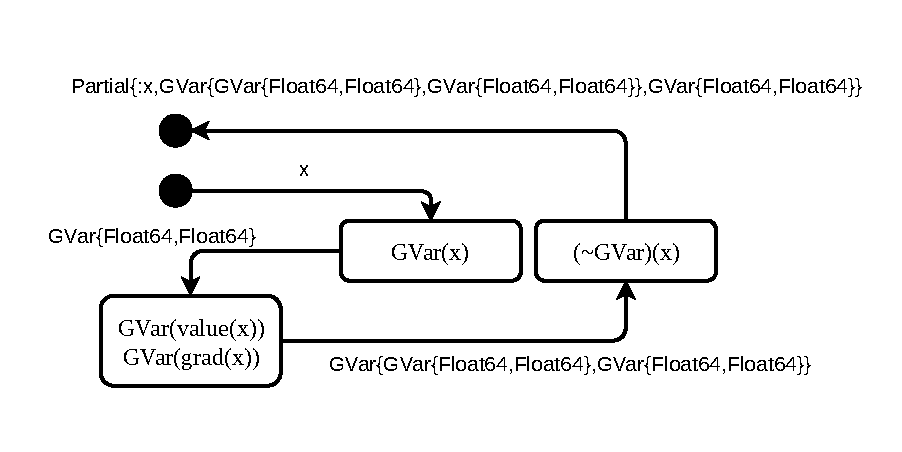
\includegraphics[width=\columnwidth,trim={0 6.5cm 1cm 2cm},clip]{images/simplehessian.pdf}}
    \caption{Obtaining the second order gradient with the reversive differentiation approach. Black lines are computing gradients, red lines are back propagating the process of obtaining the first order gradients. Annotations on lines are data types and their fields used in the computation.}\label{fig:simplehessian}
\end{figure}

\Fig{fig:simplehessian} show the four passes in computing Hessian. The first two passes (black lines) are obtaining gradients. Before entering the third pass, the program wraps each field in \texttt{GVar} with \texttt{GVar}. Then we pick a variable $x_i$ and add $1$ to \texttt{grad(grad($x_i$))} to compute the $i$-th row of Hessian. At the final stage, the \texttt{$\sim$GVar} operation does not unwrap \texttt{GVar} directly because the second order gradient fields may not be zero in this case. Instead, we use \texttt{Partial\{:x\}($\cdot$)} to safely compute \texttt{$\sim$GVar} on data type \texttt{GVar\{<:GVar, <:GVar\}}. \texttt{Partial\{:x\}} takes the \texttt{x} field of an instance without deallocating memory. By repeating the above process for different $x_i$, one can obtains the Hessian matrix.

\subsubsection{Taylor propagation}\label{sec:taylor}
A probably more efficient approach is back propagating Hessians directly~\cite{Martens2012} by
\begin{align}
    \begin{split}
        &H^{O}_{O',O''} = \mathbf{0},\\
        &H^{O}_{x,x'} = J^{y}_{x} H^{O}_{y, y'} J^{y'}_{x'} + J^{O}_{y} H^{y}_{x, x'}.
    \end{split}
\end{align}
Here, the Hessian tensor $H^O_{x,x'}$ is rank three, where the top index is often takes as a scalar and omitted.
In tensor network language, the above equation can be represented as in \Fig{fig:ad}.
Hessian propagation is a special case of Taylor propagation.
With respect to the order of gradients, Taylor propagation is exponentially more efficient in obtaining higher order gradients than differentiating lower order gradients recursively. %The later requires traversing the computational graph repeatedly.
%In JAX~\cite{Bettencourt2019}, in order to support Taylor propagation, the propagation rules for part of primitives should be manually defined.
However, the exhaused support to Taylor propagation~\cite{Bettencourt2019} requires much more effort than Jacobian propagation, this is why most AD packages choose the recursive approach.
Instruction level automatic differentiation has the advantage of having very limited primitives. It is more flexible in obtaining higher order gradients like Hessian.
An example is provided in \Sec{sec:exp}.

\subsection{Gradient on ancilla problem}
An ancilla can also carry gradient during computation. As a result, even if an ancilla can be uncomputed regoriously in the original program, its \texttt{GVar} version can not be safely uncomputed.
In these case, we simply ``drop'' the gradient field instead of raising an error. In this subsection, we prove the following theorem
\begin{theorem}
    Dropping the gradient field of an ancilla at deallocation stage does not harm the reversibility of a gradient function.
\end{theorem}
\begin{proof}
Consider a reversible function $\vy, b = f(\vx, a)$, where $a$ and $b$ are the input and output values of an ancilla. The reversibility requires $b=a$ for any $\vx$. So that
\begin{align}
    \frac{\partial b}{\partial \vx} = \vec 0.
\end{align}
In the backward pass, we discarded the gradient field of $b$.
%So the question becomes does \texttt{grad(b)} have effect on the $\vx$?
The gradient fields are derived from the values of variables, they should not have any effect to the \texttt{value} fields.
The rest is to show changing the value of \texttt{grad(b)} does not result in a different \texttt{grad.($\vx$)} in the backward pass. It can be seen from the expression the back propagation rule 
\begin{equation}
    \frac{\partial O}{\partial \vx} = \frac{\partial O}{\partial \vy}\frac{\partial \vy}{\partial \vx} + \frac{\partial O}{\partial b}\frac{\partial b}{\partial \vx},
\end{equation}
where the second term with $\frac{\partial O}{\partial{b}}$ vanishes naturally. Hence one can assume any value in the gradient field of an ancilla when entering a function, it does not have to be the discarded value.
\end{proof}
This theorem is very important to the reversibility of gradient functions, without it, the recursive differentiation scheme to obtain second order gradients can not work.
On the other side, we emphasis that although the inital value of the gradient field of an ancilla can be randomly chosen, not having a gradient field at the begining is a different story.

\section{Learn by consistency}\label{sec:train}
Consider a training task that with input $\vx^*$ and output $\vy^*$,
find a set of parameters $\vp_x$ that satisfy $\vy^* = f(\vx^*, \vp_x)$.
In traditional machine learning, we define a loss $\mathcal{L} = {\rm dist}(\vy^*, f(\vx^*, \vp_x))$ and minimize it with gradient $\frac{\partial L}{\partial \vp_x}$. This works only when the target function is locally differentiable.

Here we provide an alternative by making use of reversibility.
We construct a reversible program $\vy, \vp_y =  f_r(\vx, \vp_x)$, where $\vp_x$ and $\vp_y$ are ``garbage'' spaces which include trainable parameters and auxillary parameters.
The algorithm can be summarized as

\begin{algorithm}[H]
    \KwResult{$\vp_x$}
    Initialize $\vx$ to $\vx^*$, garbage space $\vp_x$ to random.\\
    \eIf{$\vp_y$ is \texttt{null}}{
        $\vx, \vp_x = f_r^{-1}(\vy^*)$\\
    }{
        $\vy, \vp_y= f_r(\vx, \vp_x)$\\
        \While{$\vy \not\approx \vy^*$}{
            $\vy = \vy^*$\\
            $\vx, \vp_x = f_r^{-1}(\vy, \vp_y)$.\\
            $\vx = \vx^*$\\
            $\vy, \vp_y= f_r(\vx, \vp_x)$
        }
    }
    \caption{Learn by consistency}\label{algo:train}
\end{algorithm}

Here, $\garbage(\cdot)$ is a function for taking the garbage space.
This algorithm utilizes the self-consistency relation
\begin{equation}\label{eq:selfconsistent}
    \vp_x^* = \garbage(f_r^{-1}(\vy^*, \garbage(f_r(\vx^*, \vp^*_x)))),
\end{equation}

Similar idea of training by consistency is used in self-consistent meanfield theory~\cite{Michael2003} in physics.
The difficult part of self-consistent training is to find a self-consistency relation, here the reversibility provides a natural self-consistency relation.
Learn by consistency can be used to handle descrete optimization. However, it is not a silver bullet, and should be used with causion.
Let's consider the following example

\begin{minipage}{.44\textwidth}
\begin{lstlisting}[basicstyle=\small\ttfamily,columns=fullflexible]
@i function f1(y!, x, p!)
    p! += identity(x)
    y! -= exp(x)
    y! += exp(p!)
end

@i function f2(y!, x!, p!)
    p! += identity(x!)
    y! -= exp(x!)
    x! -= log(-y!)
    y! += exp(p!)
end

function train(f)
    loss = Float64[]
    p = 1.6
    for i=1:100
        y!, x = 0.0, 0.3
        @instr f(y!, x, p)
        push!(loss, y!)
        y! = 1.0
        @instr (~f)(y!, x, p)
    end
    loss
end
\end{lstlisting}
\end{minipage}

Functions \texttt{f1} and \texttt{f2} computes $f(x, p) = e^{(p+x)} - e^x$ and stores the output in a new memory \texttt{y!}.
The only difference is \texttt{f2} ``uncompute'' $x$ arithmetically.
The task of training is to find a $p$ that make the output value equal to target value $1$.
After $100$ steps, \texttt{f2} runs into the fixed point with $x$ equal to $1$ upto machine precision.
However, \texttt{f1} does not do any training.
The training of \texttt{f2} fails because this function actually computes $\texttt{f1}(y, x, p) = y + e^{(p+x)} - e^{x}, x, x+p$, where the training parameter $p$ is completely determined by the garbage space on the output side $x \cup x+p$. As a result, shifting $y$ directly is the only approach to satisfy the consistency relation. On the other side, $\texttt{f2}(y, x, p) = y + e^{(p+x)} - e^x, \tilde{0}, x+p$, the garbage space can not uniquely determine the input garbage space $p$ and $y$. Here we use $\tilde{0}$ to denote the zero with rounding error.

\begin{figure}
    \centerline{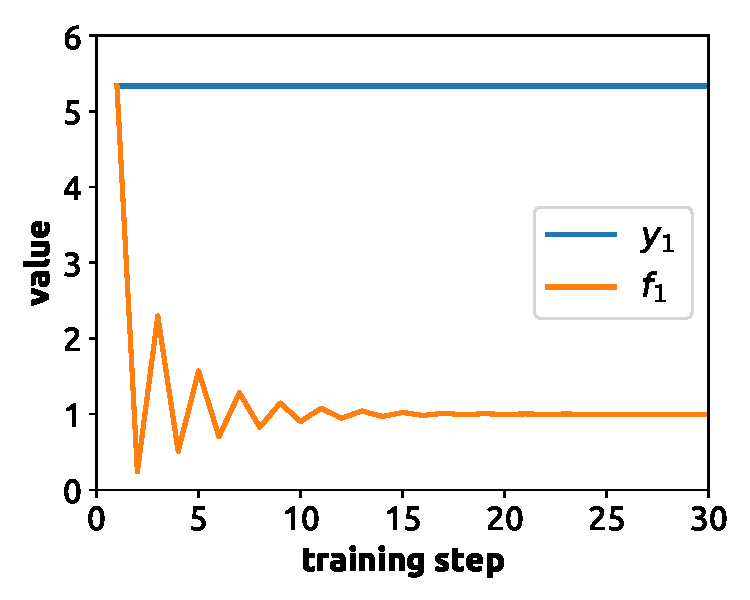
\includegraphics[width=0.9\columnwidth,trim={0 0.3cm 0 0},clip]{images/fig1.pdf}}
    \caption{The value of $x$ as a function of self-consistent training step.}\label{fig:invtrain}
\end{figure}

By viewing $\vx$ and parameters in $\vp_x$ as variables, we can study the trainability from the information perspective.
\begin{theorem}
    Only if the the conditional entropy $S(\vy|\vp_y)$ is nonzero, algorithm \ref{algo:train} is trainable.
\end{theorem}
\begin{proof}
The above example reveals a fact that the training can not work when the output $\vp_y$ completely determines $\vp_x$, that is
\begin{align}
    \begin{split}
        S(\vp_x | \vp_y) &= S(\vp_x \cup \vp_y) - S(\vp_y)\\
        &\leq S\left((\vp_x \cup \vx) \cup \vp_y \right) - S(\vp_y),\\
        &\leq S\left((\vp_y \cup \vy) \cup \vp_y\right) - S(\vp_y),\\
    &\leq S(\vy|\vp_y).
    \end{split}
\end{align}
The third line uses the bijectivity $S(\vx \cup \vp_x) = S(\vy \cup \vp_y)$.
\end{proof}
This inequality shows that when the garbage space on the output side satisfies $S(\vy | \vp_y) = 0$, i.e. contains all information to determine the output field, the input parameters are also completely determined by this garbage space.
In the above examples, it corresponds to the case $S\left(e^{(x+y)-e^x} | x \cup x + y\right) = 0$ in $f_1$.
One should remove the redundancy of information by uncomputing to make training by consistency work properly.

\section{Examples}\label{sec:example}

\subsection{Computing Fibonacci Numbers}\label{sec:fib}
An example that everyone likes

\begin{minipage}{.44\textwidth}
\begin{lstlisting}
@i function rfib(out, n::T) where T
    @anc n1 = zero(T)
    @anc n2 = zero(T)
    @routine init begin
        n1 += identity(n)
        n1 -= identity(1.0)
        n2 += identity(n)
        n2 -= identity(2.0)
    end
    if (value(n) <= 2, ~)
        out += identity(1.0)
    else
        rfib(out, n1)
        rfib(out, n2)
    end
    ~@routine init
end
\end{lstlisting}
\end{minipage}

The following example shows how to construct a reversible \texttt{while} statement. It computes the first Fibonacci number that greater or equal to $x$

\begin{minipage}{.44\textwidth}
\begin{lstlisting}
@i function rfib100(n, x)
    @safe @assert n == 0
    while (fib(n) < x, n != 0)
        n += identity(1)
    end
end
\end{lstlisting}
\end{minipage}

In this example, the postcondition \texttt{n!=0} is false before entering the loop, and becomes true in later iterations. In the reverse program, the \texttt{while} statement stops at \texttt{n==0}.

\subsection{exp function}\label{sec:exp}
An $\exp$ function can be computed using Taylor expansion
\begin{equation}
    {\rm y} += \sum\limits_n \frac{x^n}{{\rm factorial}(n)}
\end{equation}
There is a recursive algorithm to compute this expression.
The recursion relation is written as $s_n = \frac{x s_{n-1}}{n}$, where $s_{n} \equiv \frac{x^n}{{\rm factorial}(n)}$ is the term to be accumulated to $y$.
This algorithm mimics the famous pebble game~\cite{Perumalla2013}. However, there is no known constant memory and polynomial time solution to pebble game.
Here the case is different. Notice $\mathrel{*}=$ and $\mathrel{/}=$ are arithmetically reversible to each other, we can ``uncompute'' previous state $s_{n-1}$ by $s_{n-1} = \frac{n s_n}{x}$ approximately to deallocate the memory.
The implementation is

\begin{minipage}{.44\textwidth}
\begin{lstlisting}
using NiLang, NiLang.AD

@i function iexp(y!, x::T; atol::Float64=1e-14)
        where T
    @anc anc1 = zero(T)
    @anc anc2 = zero(T)
    @anc anc3 = zero(T)
    @anc iplus = 0
    @anc expout = zero(T)

    y! += identity(1.0)
    @routine r1 begin
        anc1 += identity(1.0)
        while (value(anc1) > atol, iplus != 0)
            iplus += identity(1)
            anc2 += anc1 * x
            anc3 += anc2 / iplus
            expout += identity(anc3)
            # arithmetic uncompute
            anc1 -= anc2 / x
            anc2 -= anc3 * iplus
            SWAP(anc1, anc3)
        end
    end

    y! += identity(expout)

    ~@routine r1
end
\end{lstlisting}
\end{minipage}

Here, the definition of SWAP instruction can be found in \App{app:instr}.
The two lines bellow the comment ``\texttt{\# arithmetic uncompute}'' uncompute variables \texttt{anc1} and \texttt{anc2} approximately, which is only arithmeticly true. As a result, the final output is not exact due to the rounding error. On the other side, the reversibility is not affected since the inverse call at the last line of function uncomputes all ancilla bits rigorously.
The \texttt{while} statement takes two conditions, the precondition and postconditoin. Precondition \texttt{val(anc1) > atol} indicates when to break the forward pass and post condition \texttt{iplus != 0} indicates when to break the backward pass.

To obtain gradients, one can wrap the variable \texttt{y!} with \texttt{Loss} type and feed it into \texttt{iexp\textquotesingle} or \texttt{simple\_hessian}

\begin{minipage}{.44\textwidth}
\begin{lstlisting}
julia> y!, x = 0.0, 1.6
(0.0, 1.6)

julia> @instr iexp'(Loss(y!), x)

julia> grad(x)
4.9530324244260555

julia> y!, x = 0.0, 1.6
(0.0, 1.6)

julia> simple_hessian(iexp, (Loss(y!), x))
2×2 Array{Float64,2}:
 0.0  0.0
 0.0  4.95303
\end{lstlisting}
\end{minipage}

\texttt{iexp\textquotesingle} is a callable instance of type \texttt{Grad\{typeof(iexp)\}}. \texttt{iexp\textquotesingle($\cdot$)} returns input variables with updated gradient field.
\texttt{simple\_hessian} back propagates the first order gradients to obtain Hessians as introduced in \Sec{sec:simplehessian}.
%The loss variable is specified by a wrapper \texttt{Loss}, notice we don't distinguish input and output in reversible programming.
%The gradient function is implemented reversibally so that the gradient field of output can be differentiated again to obtain Hessians as shown in \Fig{fig:simplehessian}.

A more efficient Taylor propagation approach introduced in \Sec{sec:taylor} can be accessed by feeding variables into \texttt{iexp\textquotesingle\textquotesingle}

\begin{minipage}{.44\textwidth}
\begin{lstlisting}
julia> y!, x = 0.0, 1.6
(0.0, 1.6)

julia> @instr iexp''(Loss(y!), x)

julia> collect_hessian()
2×2 Array{Float64,2}:
 0.0  0.0
 0.0  4.95303
\end{lstlisting}
\end{minipage}

\texttt{iexp\textquotesingle\textquotesingle} computes the second order gradients by wrapping variables with type \texttt{BeijingRing}~\footnote{When people ask for the location in Beijing, they will start by asking which ring.}.
Whenever an $n$-th variable or ancilla is created, we push a ring of size $2n-1$ to a global tape. Whenever an ancilla is deallocated, we pop a ring from the top. The $n$-th ring stores $H_{i\leq n,n}$ and $H_{n,i<n}$. We didn't use the symmetry relation $H_{i,j} = H_{j,i}$ to save memory here.
To simplify the implementation of backward rules described in the right most panel of \Fig{fig:ad}.
The final result can be collected by calling a global function \texttt{collect\_hessian}.

\subsection{QR decomposition}

Let's consider a slightly non-trivil function, the QR decomposition

\begin{minipage}{.44\textwidth}
\begin{lstlisting}
@i function iqr(Q, R, A::AbstractMatrix{T}) where T
    @anc anc_norm = zero(T)
    @anc anc_dot = zeros(T, size(A,2))
    @anc ri = zeros(T, size(A,1))
    for col = 1:size(A, 1)
        ri .+= identity.(A[:,col])
        for precol = 1:col-1
            idot(anc_dot[precol], Q[:,precol], ri)
            R[precol,col] +=
                identity(anc_dot[precol])
            for row = 1:size(Q,1)
                ri[row] -= anc_dot[precol] *
                    Q[row, precol]
            end
        end
        inorm2(anc_norm, ri)

        R[col, col] += anc_norm^0.5
        for row = 1:size(Q,1)
            Q[row,col] += ri[row] / R[col, col]
        end

        ~(ri .+= identity.(A[:,col]);
        for precol = 1:col-1
            idot(anc_dot[precol], Q[:,precol], ri)
            for row = 1:size(Q,1)
                ri[row] -= anc_dot[precol] *
                    Q[row, precol]
            end
        end;
        inorm2(anc_norm, ri)
        )
    end
end
\end{lstlisting}
\end{minipage}

This implementatin of QR decomposition is very naive that does not consider reorthogonalization.
\texttt{idot} and \texttt{inorm2} are functions to compute dot product and vector norm.
They are implemented as

\begin{minipage}{.44\textwidth}
\begin{lstlisting}
@i function idot(out, v1::AbstractVector{T}, v2)
        where T
    @anc anc1 = zero(T)
    for i = 1:length(v1)
        anc1 += identity(v1[i])
        CONJ(anc1)
        out += v1[i]*v2[i]
        CONJ(anc1)
        anc1 -= identity(v1[i])
    end
end

@i function inorm2(out, vec::AbstractVector{T})
        where T
    @anc anc1 = zero(T)
    for i = 1:length(vec)
        anc1 += identity(vec[i])
        CONJ(anc1)
        out += anc1*vec[i]
        CONJ(anc1)
        anc1 -= identity(vec[i])
    end
end
\end{lstlisting}
\end{minipage}

One can easily check the gradient of this naive implementation of QR decomposition is correct

\begin{minipage}{.44\textwidth}
\begin{lstlisting}
using Test
A = randn(4,4)
q = zero(A)
r = zero(A)

@i function test1(out, q, r, A)
    iqr(q, r, A)
    out += identity(q[1,2])
end

@i function test2(out, q, r, A)
    iqr(q, r, A)
    out += identity(r[1,2])
end

@test check_grad(test1, (Loss(0.0), q, r, A);
        atol=0.05, verbose=true)
@test check_grad(test2, (Loss(0.0), q, r, A);
        atol=0.05, verbose=true)
\end{lstlisting}
\end{minipage}

Here, the \texttt{check\_grad} function is a gradient checker function defined in module \texttt{NiLangCore.ADCore}.

\subsection{Unitary Matrices}\label{sec:umm}
Unitary matrices can be used to ease the gradient exploding and vanishing problem in recurrent networks~\cite{Arjovsky2015,Wisdom2016,Li2016}.
One of the simplest way to parametrize a unitary matrix is representing a unitary matrix as a product of two-level unitary operations~\cite{Li2016}. A real unitary matrix of size $N$ can be parametrized compactly by $N(N-1)/2$ rotation operations~\cite{Li2013}
\begin{align}
    {\rm ROT}(a!, b!, \theta)  = \begin{bmatrix}
        \cos(\theta) & - \sin(\theta)\\
        \sin(\theta)  & \cos(\theta)
    \end{bmatrix}
    \begin{bmatrix}
        a!\\
        b!
    \end{bmatrix},
\end{align}
where \texttt{$\theta$} is the rotation angle, \texttt{a!} and \texttt{b!} are target registers.

\begin{minipage}{.44\textwidth}
\begin{lstlisting}
@i function umm!(x, θ)
    @anc k = 0
    @anc Nin = size(x, 2)
    @anc Nout = size(x, 1)
    for j=1:Nout
        for i=Nin-1:-1:j
            k += identity(1)
            ROT(x[i], x[i+1], θ[k])
        end
    end

    # uncompute k
    for j=1:Nout
        for i=Nin-1:-1:j
            k -= identity(1)
        end
    end
end
\end{lstlisting}
\end{minipage}

%It implements the backward rule of a \texttt{ROT} instruction
%\begin{align}
%    \begin{split}
%    \overline{\theta}  &= \sum\frac{\partial R(\theta)}{\partial \theta}\odot(\overline{y}x^T)\\
%    &= \Tr\left[\frac{\partial R(\theta)}{\partial \theta}^T\overline{y}x^T\right]\\
%    &= \Tr\left[R\left(\frac{\pi}{2}-\theta\right)\overline{y}x^T\right]
%    \end{split}
%\end{align}


\section{Discussion and outlook}\label{sec:discussion}
In this paper, we introduce a Julia eDSL NiLang that simulates a reversible Turing machine (RTM).
We developed an instruction level automatic differentiation tool on this eDSL for differential programing.
It can differentiate over any program to any order reliablely and efficiently without sophisticated designs to memorize computational graph and intermediate states.
Also, we introduce a new training strategy that does not rely on gradients, learn by consistency.

In the following, we discussed the paractical side of writting reversible programs, and several future directions to go.
%Notablely, we introduce the concept of ``arithematic uncomputing'' to reduce the overhead of recursive reversible algorithms.

\subsection{Time Space Tradeoff}\label{sec:timespace}
In history, there has been many other designs of reversible languages and instruction sets.
One of the main reason why RTM is not so popular is it may have either a space overhead propotional to computing time $T$ or a computational overhead that sometimes can be even exponential.
In the simplest g-segment trade off scheme~\cite{Bennett1989,Levine1990},
\begin{align}
    Time(T) &= \frac{T^{1+\epsilon}}{S^\epsilon}\\
    Space(T) &= \epsilon 2^{1/\epsilon}(S+S\log\frac{T}{S})
\end{align}
with $T$ and $S$ the time and space usage on a irreversible Turing machine, $\epsilon$ is the control parameter.
It is related to the g-segment trade off parameters by $g = k^n, \epsilon = \log_k(2k-1)$ with $n\geq 1$ and $k\geq 1$.
This section, we try to convince the readers that the overhead of reversible computing is not as terrible as people thought.

First, at $\epsilon \rightarrow 0$, the resource used by a RTM is same as the caching stategy used in a traditional machine learning package that memorizing every inputs of primitives. Memorizing inputs always make a program reversible since it does not discard any information.
For deep neural networks, people used checkpointing trick to trade time with space~\cite{Chen2016}, which is also a widely used trick in reversible programming~\cite{Perumalla2013}. RTM just provides more alternatives to trade time and space.

%For inplace functions, especially those reversible functions. Reversible programming AD is sometimes more memory efficient. Comparing with logging computational graph.
Second, some computational overhead of running recursive algorithms with limited space resources can be mitigated by "pseudo uncomputing" without sacrifising reversibility like in the \texttt{iexp} example. With reversible floating point $\mathrel{*}=$ and $\mathrel{/}=$ operations~\cite{Hner2018}, many primitives can be implemented with pure reversible functions, which may significant decrease the computation time and memory usage. We will review this point in \Sec{sec:hardware}.

Third, making reversible programming an eDSL rather than a independant language allows flexible choices between reversibility and computational overhead. For example, in order to deallocate the gradient memory in a reversible language one has to uncompute the whole process of obtaining this gradient.
As a reversible eDSL, we have the flexibility to deallocate the memory irreversibly, i.e. trade energy with time. To quantify the overhead of uncomputing, we introducing the concept
\begin{definition}[program granularity]
    The logarithm of the ratio between the execution time of a reversible program and its irreversible counter part.
    \begin{equation}
        \log_2 \frac{Time(T)}{T}
    \end{equation}
\end{definition}
Whenever the program uncomputes the memory, the program granularity increases by approximately one. In instruction design, defining primitive functions like \texttt{iexp}, and deallocating gradients used for training, we need uncomputing ancilla bits and increase the granularity. The overhead increase exponentially as the granuality increase.
The granularity can be decreased by cleverer compilation of a program, since the uncomputing of ancillas can be executed at any level of abstraction.

%One should notice the memory advantage of reversible programming to machine learning does comes from reversibility itself, but from a better data tracking strategy inspired from invertible programming.
%Normally, a reversible program is not as memory efficient as its irreversible couterpart due to the additional requirement of no information loss. A naive approach that keeping track of all informations will cost an additional space $O(T)$, where $T$ stands for the excution time in a irreversible TM, the longer the program runs, the larger the memory usage is. This is exactly the approach to keeping reversibility in most machine learning packages in the market.
%The point it, an reversible Turing Machine is able to trade space with time.
%In some cases, it may cause polynomial overhead than its irreversible counterpart.

\subsection{Instructions and Hardwares}\label{sec:hardware}
%Todays CPU are starving, that is, the memory access is the performance bottleneck in many applications rather than the arithmetic operations.
%There is a natural granularity for operations with memory access or not.
So far, our eDSL is not really compiled to instructions, instead, it runs on a irreversible host Julia.
In the future, it can be compiled to low level instructions and is execute on a reversible devices.
For example, the control flow defined in this NiLang can be compiled to reversible instructions like conditioned \texttt{goto} instruction.
The reversibility requires the target instruction a \texttt{comefrom} instruction that specifing the postcondition. ~\cite{Vieri1999}

Arithmetic instructions should be redesigned to support better reversible programs.
The major obstacle to exact reversibility programming is current floating point adders used in our computing devices are not exactly reversible.
There are proposals of reversible floating point adders and multipliers~\cite{Nachtigal2010,Nachtigal2011,Nguyen2013,Hner2018} that introduces garbage bits to ensure reversibility.
%In other words, to represent a 64 bit floating point number requires more than 64 bits in storage. Reversible multiplier is also possible in similar approach.~\cite{Nachtigal2010} 
With these infrastructure, a reversibile program can be executed without suffereing from the irreversibility from rounding error and reduce the computational and memory overhead significantly.
Notablely, in machine learning field, information buffer is used to make multiplication operations~\cite{Maclaurin2015} reversible and reduce memory cost.

Reversible programming is not nessesarily related to reversible hardwares. Reversible programs are a subset of irreversible programs, hence can be simulated efficiently on CMOS devices~\cite{Vieri1999}. By Using reversible hardwares~\cite{}, the computation may costs zero energy by Landauer's principle~\cite{Landauer1961}.
Reversible hardwares are not nessesarily related to reversible gates such as Toffoli gate and Fredkin gate.
Devices with the ability of recovering signal energy is able able to save energy, which is known as generalized reversible computing.~\cite{Frank2005,Frank2017b}
In the following, we comment briefly on a special type of reversible device Quantum computer.

\subsubsection{Quantum Computers}\label{sec:qc}
One of the fundamental difficulty of building a quantum computer is, unlike a classical state, an unknown quantum state can not be copied.
Quantum random access memory~\cite{Giovannetti2008} is very hard to design and implement, which is known to have many caveats~\cite{Aaronson2015}.
A quantum state in a environment will decoherence and can not be recovered, this underlines the simulation nature of quantum devices.
%In the era of noisy intermediate sized quantum devices, more and more people are switching to classical-quantum hybrid devices, where a quantum device plays the role of a programmable simulator.
Reversible computing does not enjoy the quantum advantage, nor the quantum disadvantages of non-cloning and decoherence.
The reversibility of quantum computing comes from the fact that microscopic processes are unitary.
On the other side, the irreversibility is rare, it can come from interacting with classical devices. Irreversible processes include decaying, qubit state resetting, measurements and classical feedbacks to quantum devices. These are typically harder to implement on a quantum device.

Given the fundamental limitations of quantum decoherence and non-cloning and the reversible nature of microscopic world.
It is reasonable to have a reversible computing device to bridge the gap between classical and universal quantum computing.
By introducing entanglement little by little, we can accelerate some basic components. For example, quantum Fourier transformation provides an interesting alternative to the adders and multipliers by introducing one additional CPHASE gate even though it is a classical-in classical-out algorithm.~\cite{RuizPerez2017}
By introducing qantum rotation gates $R_y(\theta)$ and $R_z(\theta)$ in the reversible programming, we make NiLang a path integral based universal quantum simulator as shown in \App{app:quantum}. The compiling theory developed for reversible programming will have profounding effect to quantum computing.

\subsection{Outlook}\label{sec:outlook}
So far NiLang is not full ready for productivility. It can be improved from multiple perspectives. We call for better compiling that decreases granularity and hence reduces overhead, rigoriously reversible floating point arithematics to let the reversibility free from rounding error. It is also interesting to see how it can be combined with a high performance quantum simulator like Yao~\cite{Luo2019}. It can provide control flow to Yao's quantum block intermediate representation, while Yao can provide the quantum features for NiLang.
% By porting a quantum simulator. 
%it is interesting to see how quantum simulator can improve the instruction design. Notice a quantum fourier transformation (QFT) based quantum adder and multiplier is sometimes more efficient than a classical adder~\cite{Haener2018} \blue{Is this true?}.
Reversible programming is known to have advantage in parallel computingi in handle asynchronious computing~\cite{Jefferson1985} and debugging with bidirectional move~\cite{Boothe2000}.
It is interesting to see how NiLang combines with other parts of Julia ecosystem like CUDAnative~\cite{Besard2018} and Debugger.
%This could be used to reduce the momory cost in normalizing flow, time reversible integrator, recurrent neural network and residual neural network.

\section{acknowledgments}
Jin-Guo Liu thank Lei Wang for motivating the project with possible applications reversible integrator, normalizing flow and neural ODE.
Xiu-Zhe Luo for discussion on the implementation details of source to source automatic differetiation,
Shuo-Hui Li for helpful discussion on differential geometry.
Damian Steiger for telling me the \texttt{comefrom} joke.
Tong Liu and An-Qi Chen for helpful discussion on quantum adders and multipliers.
The authors are supported by the National Natural Science Foundation of China under the Grant No.~11774398, the Strategic Priority Research Program of Chinese Academy of Sciences Grant No.~XDB28000000 and the research funding from Huawei Technologies under the Grant No.~YBN2018095185.

\bibliographystyle{apsrev4-1}
\bibliography{invc}

\pagebreak
\appendix

\section{NiLang Grammar}\label{app:grammar}

Terminologies
\begin{itemize}
    \item $ident$, symbols
    \item $num$, numbers
    \item $\epsilon$, empty statement
    \item $JuliaExpr$, native julia expression
    \item $[$ $]$,  zero or one repetitions.
\end{itemize}

\begin{minipage}{0.3\textwidth}
    \small
\begin{bnf*}
    \bnfprod{Stmts}{\bnfsp \bnfes}\\
    \bnfmore{\bnfor \bnfpn{Stmt}}\\
    \bnfmore{\bnfor \bnfpn{Stmts} \bnfsp \bnfpn{Stmt}}\\
    \bnfprod{Stmt}{\bnfpn{BlockStmt}}\\
    \bnfmore{\bnfor \bnfpn{IfStmt}}\\
    \bnfmore{\bnfor \bnfpn{WhileStmt}}\\
    \bnfmore{\bnfor \bnfpn{ForStmt}}\\
    \bnfmore{\bnfor \bnfpn{InstrStmt}}\\
    \bnfmore{\bnfor \bnfpn{RevStmt}}\\
    \bnfmore{\bnfor \bnfpn{@anc} \bnfsp \bnfpn{Stmt}}\\
    \bnfmore{\bnfor \bnfpn{@routine} \bnfsp \bnfpn{Stmt}}\\
    \bnfmore{\bnfor \bnfpn{@safe} \bnfsp \bnftd{$JuliaExpr$}}\\
    \bnfmore{\bnfor \bnfpn{CallStmt}}\\
    \bnfprod{BlockStmt}{\bnftd{begin} \bnfsp \bnfpn{Stmts} \bnfsp \bnftd{end}}\\
    \bnfprod{RevCond}{\bnftd{(} \bnfsp \bnftd{$JuliaExpr$} \bnfsp \bnftd{,} \bnfsp \bnftd{$JuliaExpr$} \bnfsp \bnftd{)}}\\
    \bnfprod{IfStmt}{\bnftd{if} \bnfsp \bnfpn{RevCond} \bnfsp \bnfpn{Stmts} \bnfsp \bnfts{[} \bnftd{else} \bnfsp \bnfpn{Stmts}\bnfts{]} \bnfsp \bnftd{end}}\\
    \bnfprod{WhileStmt}{\bnftd{while} \bnfsp \bnfpn{RevCond} \bnfsp \bnfpn{Stmts} \bnfsp \bnftd{end}}\\
    \bnfprod{Range}{\bnftd{$JuliaExpr$} \bnfsp \bnftd{:} \bnfsp \bnftd{$JuliaExpr$} \bnfsp \bnfts{[} \bnftd{:} \bnfsp \bnftd{$JuliaExpr$}\bnfts{]}}\\
    \bnfprod{ForStmt}{\bnftd{for} \bnfsp \bnftd{ident} \bnfsp \bnftd{=} \bnfsp \bnfpn{Range} \bnfsp \bnfpn{Stmts} \bnfsp \bnftd{end}}\\
    \bnfprod{CallStmt}{\bnftd{$JuliaExpr$} \bnfsp \bnftd{(} \bnfsp \bnfts{[} \bnfpn{DataViews}\bnfts{]} \bnfsp \bnftd{)}}\\
    \bnfprod{Constant}{\bnftd{num} \bnfor \bnftd{$\pi$}}\\
    \bnfprod{InstrBinOp}{\bnftd{+=} \bnfor \bnftd{-=} \bnfor \bnftd{$\veebar$=}}\\
    \bnfprod{InstrTrailer}{\bnfts{[} \bnftd{.}\bnfts{]} \bnfsp \bnftd{(} \bnfsp \bnfts{[} \bnfpn{DataViews}\bnfts{]} \bnfsp \bnftd{)}}\\
    \bnfprod{InstrStmt}{\bnfpn{DataView} \bnfsp \bnfpn{InstrBinOp} \bnfsp \bnftd{ident} \bnfsp \bnfts{[} \bnfpn{InstrTrailer}\bnfts{]}}\\
    \bnfprod{RevStmt}{\bnftd{$\sim$} \bnfsp \bnfpn{Stmt}}\\
    \bnfprod{@routine}{\bnftd{@routine} \bnfsp \bnftd{ident} \bnfsp \bnfpn{Stmt}}\\
    \bnfprod{AncArg}{\bnftd{ident} \bnfsp \bnftd{=} \bnfsp \bnftd{$JuliaExpr$}}\\
    \bnfprod{@anc}{\bnftd{@anc} \bnfsp \bnfpn{AncArg}}\\
    \bnfmore{\bnfor \bnftd{@deanc} \bnfsp \bnfpn{AncArg}}\\
    \bnfprod{@safe}{\bnftd{@safe} \bnfsp \bnftd{$JuliaExpr$}}\\
    \bnfprod{DataViews}{\bnfsp \bnfes}\\
    \bnfmore{\bnfor \bnfpn{DataView}}\\
    \bnfmore{\bnfor \bnfpn{DataViews} \bnfsp \bnftd{,} \bnfsp \bnfpn{DataView}}\\
    \bnfprod{DataView}{\bnfpn{DataView} \bnfsp \bnftd{[} \bnfsp \bnftd{$JuliaExpr$} \bnfsp \bnftd{]}}\\
    \bnfmore{\bnfor \bnfpn{DataView} \bnfsp \bnftd{.} \bnfsp \bnftd{ident}}\\
    \bnfmore{\bnfor \bnftd{$JuliaExpr$} \bnfsp \bnftd{(} \bnfsp \bnfpn{DataView} \bnfsp \bnftd{)}}\\
    \bnfmore{\bnfor \bnfpn{Constant}}\\
    \bnfmore{\bnfor \bnftd{ident}}\\
\end{bnf*}

\end{minipage}

One can use \texttt{@i function $\<Stmts\>$ end} to define a function and its inverse. All $JuliaExpr$ is should be pure, otherwise the reversibility is not gurantted.

Dataview is a bijective mapping of an object or a field (or item) of an object.
When modifying the dataview of an object, it changes the object directly with the \texttt{chfield} method.

\section{Instruction Table}\label{app:instr}

The translation of instructions to Julia functions
\begin{table}[h!]\centering
\begin{minipage}{\columnwidth}
\ra{1.3}
    \scalebox{1.0}{
        \begin{tabularx}{\textwidth}{X X X}\toprule
            \textbf{instruction} & \textbf{translated} & \textbf{type}\\
            \hline
            $y \pluseq f(args...)$ & $\oplus(f)(args...)$ & \texttt{PlusEq}\\
            $y \minuseq f(args...)$ & $\ominus(f)(args...)$ & \texttt{MinusEq}\\
            $y \mathrel{\veebar}= f(args...)$ & $\odot(f)(args...)$ & \texttt{XorEq}\\
            \bottomrule
        \end{tabularx}
    }
    \caption{Instructions and their interpretation in NiLang.}\label{tbl:interp}
\end{minipage}
\end{table}


The list of instructions implemented in NiLang
\begin{table}[h!]\centering
\begin{minipage}{\columnwidth}
\ra{1.3}
    \scalebox{1.0}{
        \begin{tabularx}{\textwidth}{X X}\toprule
            \textbf{instruction} & \textbf{output}\\
            \hline
            ${\rm SWAP}(a, b)$ & $b, a$\\
            ${\rm ROT}(a, b, \theta)$ & $a \cos\theta - b\sin\theta, b \cos\theta + a\sin\theta, \theta$\\
            ${\rm IROT}(a, b, \theta)$ & $a \cos\theta + b\sin\theta, b \cos\theta - a\sin\theta, \theta$\\
            $y \pluseq a^\wedge b$ & $y+a^b, a, b$\\
            $y \pluseq \exp(x)$ & $y+e^x, x$\\
            $y \pluseq \log(x)$ & $y+\log x, x$\\
            $y \pluseq \sin(x)$ & $y+\sin x, x$\\
            $y \pluseq \cos(x)$ & $y+\cos x, x$\\
            $y \pluseq {\rm abs}(x)$ & $y+ |x|, x$\\
            ${\rm NEG}(y)$ & $-y$\\
            ${\rm CONJ}(y)$ & $y'$\\
            \bottomrule
        \end{tabularx}
    }
    \caption{A collection of reversible instructions, ``.'' is the broadcast operations in Julia.}\label{tbl:revinstructions}
\end{minipage}
\end{table}


\end{document}
